\section{Exemplos}

\begin{frame}[fragile]{Exemplo: Esvaziar o registrador $R_n$}

    O programa a seguir, que consiste em uma única instrução, esvazia o conteúdo do registrador
    $R_n$:
    \begin{small}
    \[
        (1)\ \ \left\lbrace \begin{array}{ll}
                    \mbox{se $[n]$ é diferente de zero},& \mbox{então subtraia um e permaneça em $1$}\\
                    \mbox{se $[n]$ é igual a zero},& \mbox{então pare}\\
                \end{array}\right.
    \]
    \end{small}

    \renewcommand{\figurename}{Exemplo}
    \begin{figure}[ht]
        \centering
        \begin{subfigure}{.45\textwidth}
            \centering
            \caption{Fluxograma}
            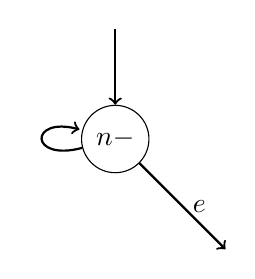
\begin{tikzpicture}[scale=0.7]
                \coordinate (A) at (0, 4);
                \node[draw,circle] (B) at (0, 2) { $n-$ };
                \coordinate (C) at (-2, 0);
                \coordinate (D) at (2, 0);

                \draw[thick,->] (A) -- (B);
                \draw[thick,->] (B) edge[loop left] (B);
                \draw[thick,->] (B) -- node[anchor=west] { $e$ } (D);
            \end{tikzpicture}
        \end{subfigure}
        \begin{subfigure}{.45\textwidth}
            \centering
            \caption{Diagrama de Blocos}
            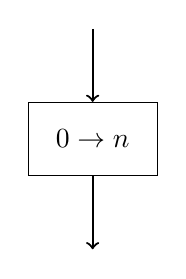
\begin{tikzpicture}[scale=0.7]
                \coordinate (A) at (0, 4);
                \node[draw,minimum size=10pt,inner sep=10pt] (B) at (0, 2) { $0 \to n$ };
                \coordinate (C) at (0, 0);

                \draw[thick,->] (A) -- (B);
                \draw[thick,->] (B) -- (C);
            \end{tikzpicture}
        \end{subfigure}
        \caption{Esvaziar o registrador $R_n$}
    \end{figure}
\end{frame}

\begin{frame}[fragile]{Exemplo: Esvaziar o registrador $R_m$ no registrador $R_n$}

    O programa abaixo esvazia o conteúdo do registrador $R_m$ no registrador $R_n$, assumindo
    que ambos registradores são distintos.

    \renewcommand{\figurename}{Exemplo}
    \begin{figure}[ht]
        \centering
        \begin{subfigure}{.45\textwidth}
            \centering
            \caption{Fluxograma}
            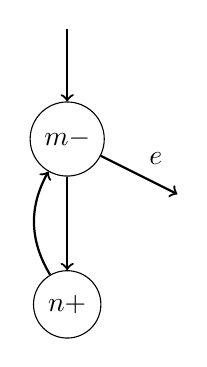
\begin{tikzpicture}[scale=0.7]
                \coordinate (A) at (0, 4);
                \node[draw,circle] (B) at (0, 2) { $m-$ };
                \node[draw,circle] (C) at (0, -1) { $n+$ };
                \coordinate (D) at (2, 1);

                \draw[thick,->] (A) -- (B);
                \draw[thick,->] (B) -- (C);
                \draw[thick,->] (C) edge[bend left] (B);
                \draw[thick,->] (B) -- node[anchor=south west] { $e$ } (D);
            \end{tikzpicture}
        \end{subfigure}
        \begin{subfigure}{.45\textwidth}
            \centering
            \caption{Diagrama de Blocos}
            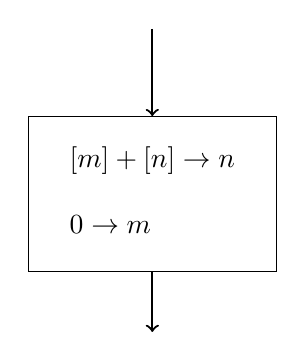
\begin{tikzpicture}[scale=0.7]
                \coordinate (A) at (0, 5);
                \node[draw,minimum size=10pt,inner sep=10pt] (B) at (0, 2) { 
                    $\begin{array}{ll} [m] + [n] \to n \\ \\ 0 \to m\end{array}$ };
                \coordinate (C) at (0, -0.5);

                \draw[thick,->] (A) -- (B);
                \draw[thick,->] (B) -- (C);
            \end{tikzpicture}
        \end{subfigure}
        \caption{Esvaziar $R_m$ em $R_n$}
    \end{figure}
\end{frame}

\begin{frame}[fragile]{Exemplo: Adicionar $R_m$ a $R_n$, sem perda de $R_m$}

    Para adicionar o conteúdo de $R_m$ em $R_n$, sem perda de $R_m$, é preciso um registrador
    auxiliar $R_p$, inicialmente vazio.

    \renewcommand{\figurename}{Exemplo}
    \begin{figure}[ht]
        \centering
        \begin{subfigure}{.55\textwidth}
            \centering
            \caption{Fluxograma}
            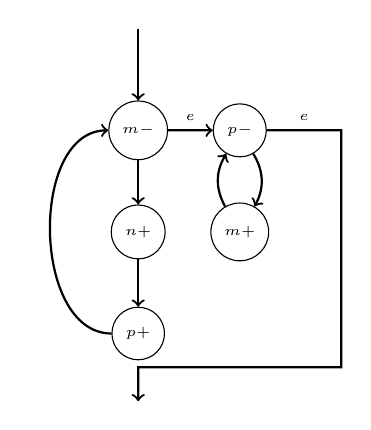
\begin{tikzpicture}[scale=0.43]
                \coordinate (A) at (0, 9);
                \node[draw,circle] (B) at (0, 6) { \tiny $m-$ };
                \node[draw,circle] (C) at (0, 3) { \tiny $n+$ };
                \node[draw,circle] (D) at (0, 0) { \tiny $p+$ };
                \coordinate (E) at (0, -1);
                \coordinate (F) at (0, -2);

                \node[draw,circle] (X) at (3, 6) { \tiny $p-$ };
                \node[draw,circle] (Y) at (3, 3) { \tiny $m+$ };

                \coordinate (M) at (6, 6);
                \coordinate (N) at (6, -1);

                \draw[thick,->] (A) -- (B);
                \draw[thick,->] (B) -- (C);
                \draw[thick,->] (C) -- (D);
                \draw[thick,->] (D) edge[in=180,out=180] (B);

                \draw[thick,->] (B) -- node[anchor=south] { \tiny $e$ } (X);
                \draw[thick,->] (X) edge[bend left] (Y);
                \draw[thick,->] (Y) edge[bend left] (X);

                \draw[thick,->] (X) -- node[anchor=south] { \tiny $e$ } (M) -- (N) -- (E) -- (F);
            \end{tikzpicture}
        \end{subfigure}
        \begin{subfigure}{.35\textwidth}
            \centering
            \caption{Diagrama de Blocos}
            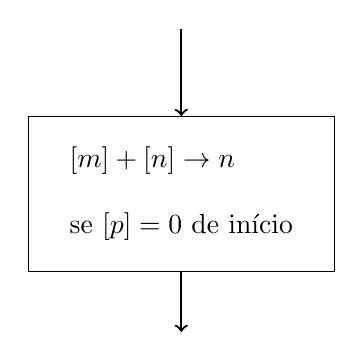
\begin{tikzpicture}[scale=0.7]
                \coordinate (A) at (0, 5);
                \node[draw,minimum size=10pt,inner sep=10pt] (B) at (0, 2) { 
                    $\begin{array}{ll} [m] + [n] \to n \\ \\ \mbox{se}\ [p] = 0\ \mbox{de início}\end{array}$ };
                \coordinate (C) at (0, -0.5);

                \draw[thick,->] (A) -- (B);
                \draw[thick,->] (B) -- (C);
            \end{tikzpicture}
        \end{subfigure}
        \caption{Adicionar $R_m$ a $R_n$, sem perda de $R_m$}
    \end{figure}
\end{frame}

\begin{frame}[fragile]{Exemplo: Multiplicação}

    O ábaco abaixo computa o produto dos números armazenados em $R_a$ e $R_b$. O resultado ficará
    armazenado em $R_n$ e, inicialmente, tanto $R_n$ quanto $R_p$ devem estar vazios.

    \renewcommand{\figurename}{Exemplo}
    \begin{figure}[ht]
        \centering
        \begin{subfigure}{.45\textwidth}
            \centering
            \caption{Fluxograma abreviado}
            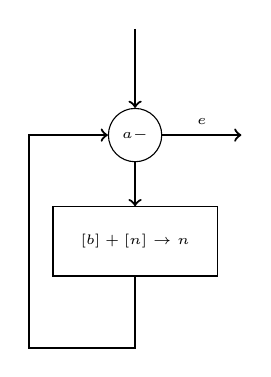
\begin{tikzpicture}[scale=0.45]
                \coordinate (A) at (0, 9);
                \node[draw,circle] (B) at (0, 6) { \tiny $a-$ };
                \node[draw,minimum size=10pt,inner sep=10pt] (C) at (0, 3) { \tiny $[b] + [n]\to n$ };
                \coordinate (D) at (0, 0);
                \coordinate (X) at (-3, 0);
                \coordinate (Y) at (-3, 6);
                \coordinate (Z) at (3, 6);

                \draw[thick,->] (A) -- (B);
                \draw[thick,->] (B) -- (C);
                \draw[thick,->] (C) -- (D) -- (X) -- (Y) -- (B);
                \draw[thick,->] (B) -- node[anchor=south] { \tiny $e$ } (Z);
            \end{tikzpicture}
        \end{subfigure}
        \begin{subfigure}{.45\textwidth}
            \centering
            \caption{Diagrama de Blocos}
            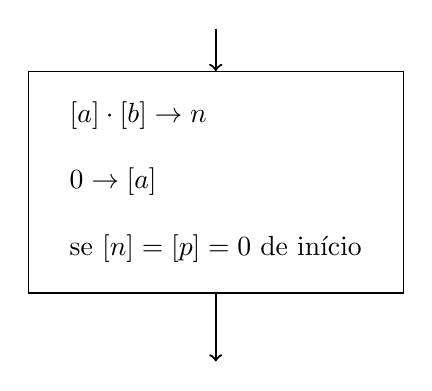
\begin{tikzpicture}[scale=0.65]
                \coordinate (A) at (0, 5);
                \node[draw,minimum size=10pt,inner sep=10pt] (B) at (0, 2) { 
                    $\begin{array}{ll} [a] \cdot [b] \to n \\ \\0\to [a]\\ \\ \mbox{se}\ [n] = [p] = 0\ \mbox{de início}\end{array}$ };
                \coordinate (C) at (0, -1.5);

                \draw[thick,->] (A) -- (B);
                \draw[thick,->] (B) -- (C);
            \end{tikzpicture}
        \end{subfigure}
        \caption{Multiplicar $R_a$ e $R_b$}
    \end{figure}
\end{frame}

\begin{frame}[fragile]{Exemplo: Multiplicação}

    \begin{figure}[ht]
        \centering
        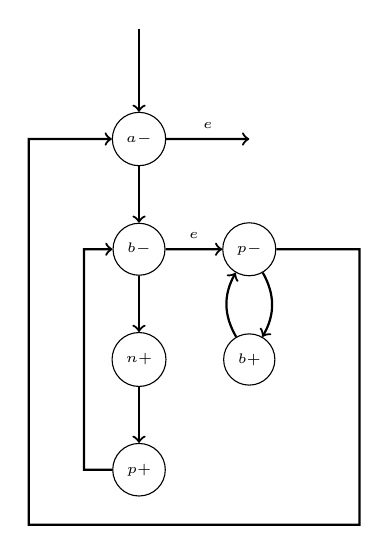
\begin{tikzpicture}[scale=0.7]
            \coordinate (A) at (0, 10);
            \node[draw,circle] (B) at (0, 8) { \tiny $a-$ };
            \node[draw,circle] (C) at (0, 6) { \tiny $b-$ };
            \node[draw,circle] (D) at (0, 4) { \tiny $n+$ };
            \node[draw,circle] (E) at (0, 2) { \tiny $p+$ };

            \coordinate (X) at (-1, 2);
            \coordinate (Y) at (-1, 6);

            \coordinate (L) at (2, 8);
            \node[draw,circle] (M) at (2, 6) { \tiny $p-$ };
            \node[draw,circle] (N) at (2, 4) { \tiny $b+$ };

            \coordinate (P) at (4, 6);
            \coordinate (Q) at (4, 1);
            \coordinate (R) at (-2, 1);
            \coordinate (S) at (-2, 8);

            \draw[thick,->] (A) -- (B);
            \draw[thick,->] (B) -- (C);
            \draw[thick,->] (C) -- (D);
            \draw[thick,->] (D) -- (E);
            \draw[thick,->] (E) -- (X) -- (Y) -- (C);

            \draw[thick,->] (B) -- node[anchor=south] { \tiny $e$ } (L);
            \draw[thick,->] (C) -- node[anchor=south] { \tiny $e$ } (M);
            \draw[thick,->] (M) edge[bend left] (N);
            \draw[thick,->] (N) edge[bend left] (M);
        
            \draw[thick,->] (M) -- (P) -- (Q) -- (R) -- (S) -- (B);
        \end{tikzpicture}
        \caption{Fluxograma completo}
    \end{figure}

\end{frame}
